\subsection{Integration auf Applikationsebene}
für Middle-Tier

Punkt-zu-Punkt-Integrationen führt zur Verwaltung von x Schnittstellen

\begin{itemize}
    \item API, EAI, B2x
    \item Service-Oriented Architecture (SOA) ist eine Voraussetzung
    \item \textcolor{blue}{Technische Heterogenität} der Plattformen unterschiedlicher Systeme überwinden und auch Legacy Systeme miteinbeziehen
    \item Cloud-Services und Social Media Services integrieren
    \item Begrifflichkeiten und Schwerpunkte der Fachdomänen berücksichtigen und Übersetzungslayer vorsehen
    \item Schnittstellen mit Spezifikationen und Mapping-Informationen verwalten
    \item Integrations-Middleware auswählen
    \item Wahl der Transportprotokolle, sowie Message-Normen
\end{itemize}
\vspace{10pt}

\subsubsection{Schnittstellen}

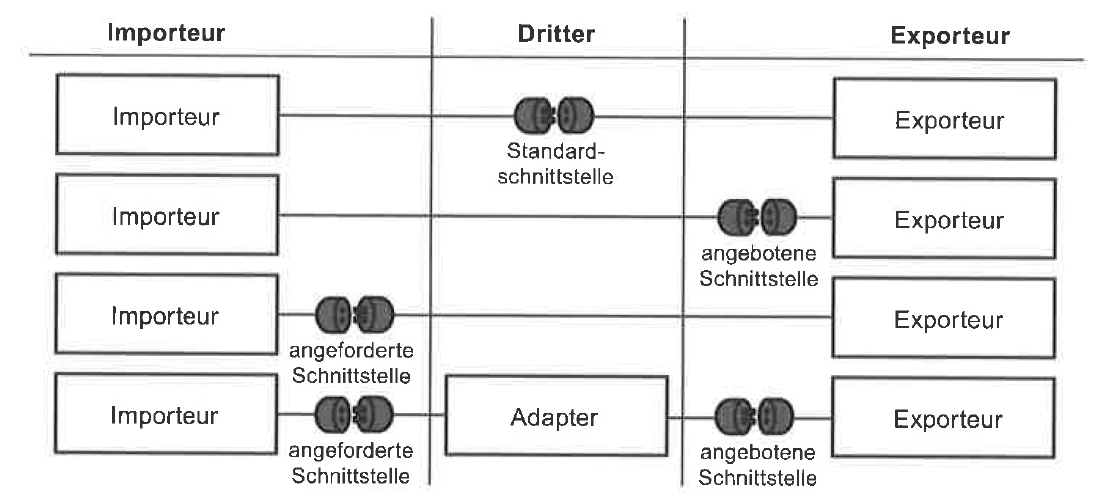
\includegraphics[width=\linewidth]{integration-contract.png} \\

\textbf{Adapter}

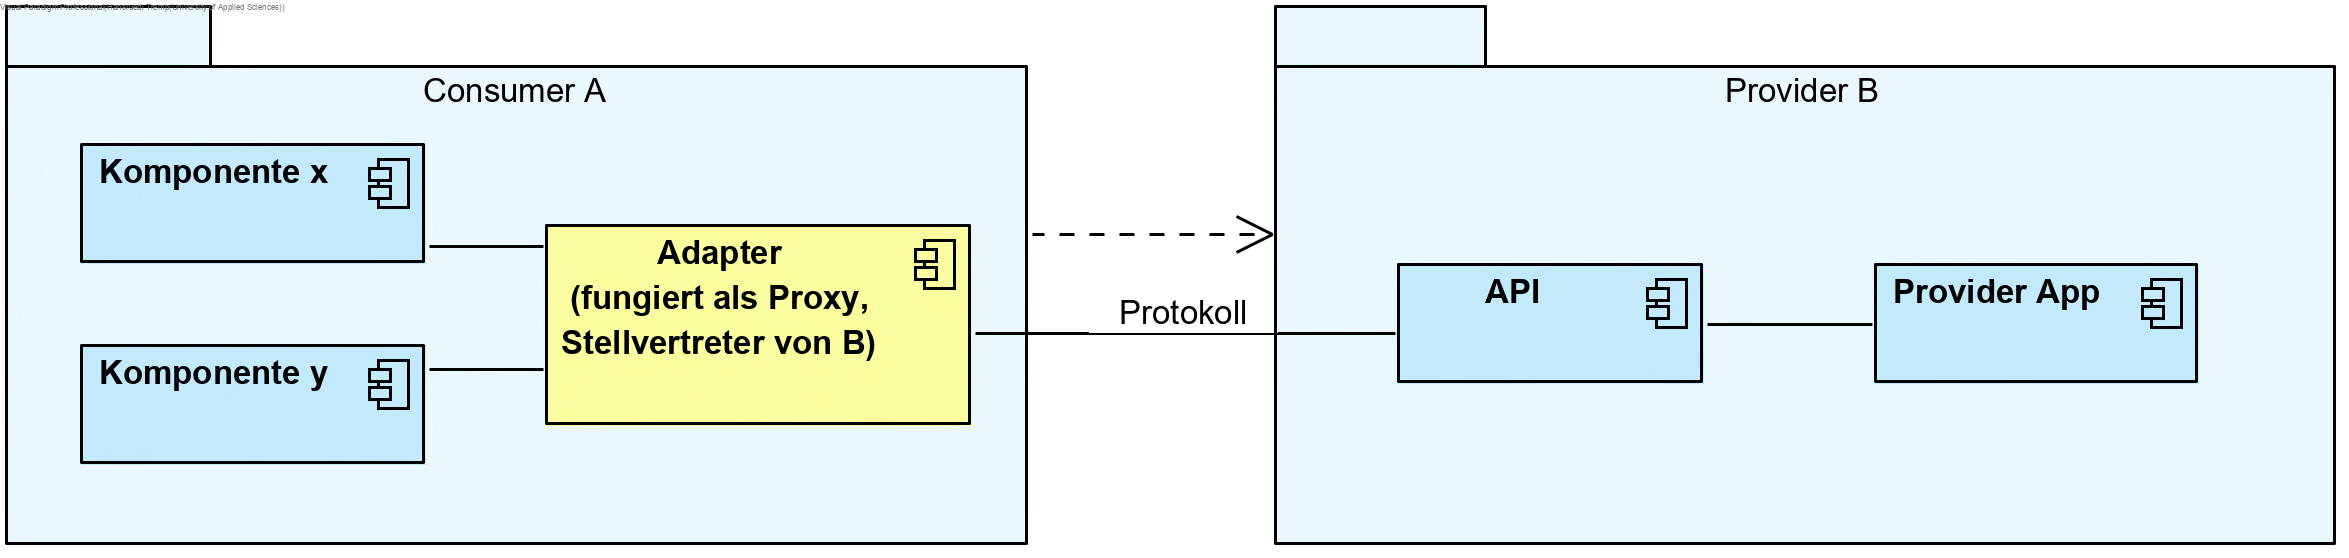
\includegraphics[width=\linewidth]{integration-adapter.png} \\

\begin{itemize}
    \item \textcolor{blue}{API} Application Programming Interface, Port (Adressierung)
    \item \textcolor{blue}{Adapter (Konnektor)} enthält alle Spezifika einer Schnittstelle, fungiert als Proxy (Stellvertreter)
\end{itemize}
\vspace{10pt}
\textbf{Gateway}

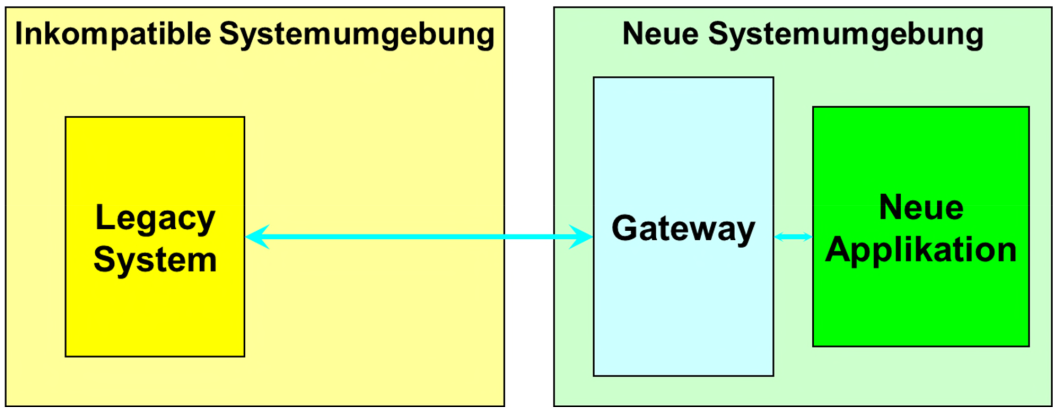
\includegraphics[width=\linewidth]{integration-gateway.png} \\

\textbf{Wrapper}

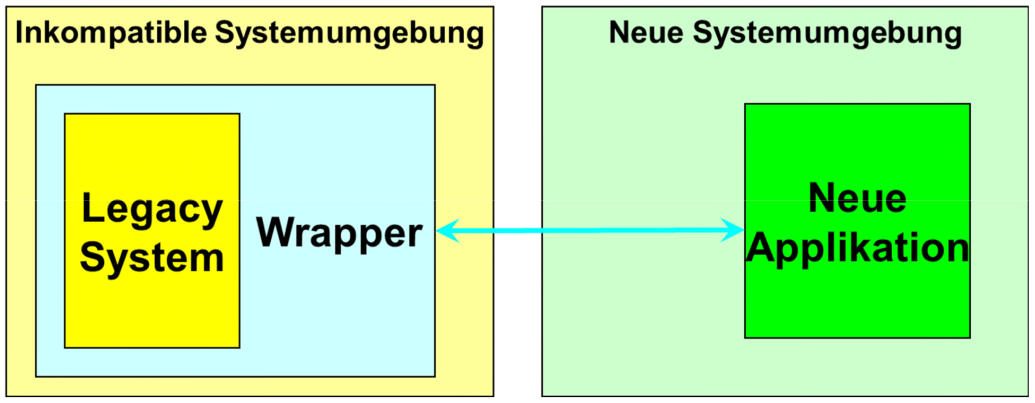
\includegraphics[width=\linewidth]{integration-wrapper.png} \\

\textbf{Integration Middleware (IM)}

bietet zwischen organisationsinternen und externen Applikationen einen workflowgetriebenen automatischen Datenaustausch (Integration-Broker).

bildet die Datendrehscheibe der Organisation, sie bietet die passenden APIs für alle internen Apps, wie Fach- und Querschnittsapplikationen an \\

\textcolor{blue}{APIs für...}

\begin{itemize}
    \item Kommunikationsdienst
    \item Transformationsdienst
    \item Datenroutingdienst
    \item Workflowdienst
    \item Monitoringdienst
\end{itemize}
\vspace{10pt}
\textcolor{blue}{Funktionen}

\begin{itemize}
    \item Connectivity zu Umsystemen über Standard-Konnektoren
    \item Synchrone Echtzeitverarbeitung mittels API-Gateway
    \item Asynchrones Messaging über Message-Broker
    \item Messagekonversion mittels Datenmapping und Codekonversionen
    \item Modellierung von Integrations-Workflows
\end{itemize}

\subsubsection{Integrationsarchitekturentwurf (Modellierung)}

Beschreibung einer Applikationsschnittstelle (Notation)

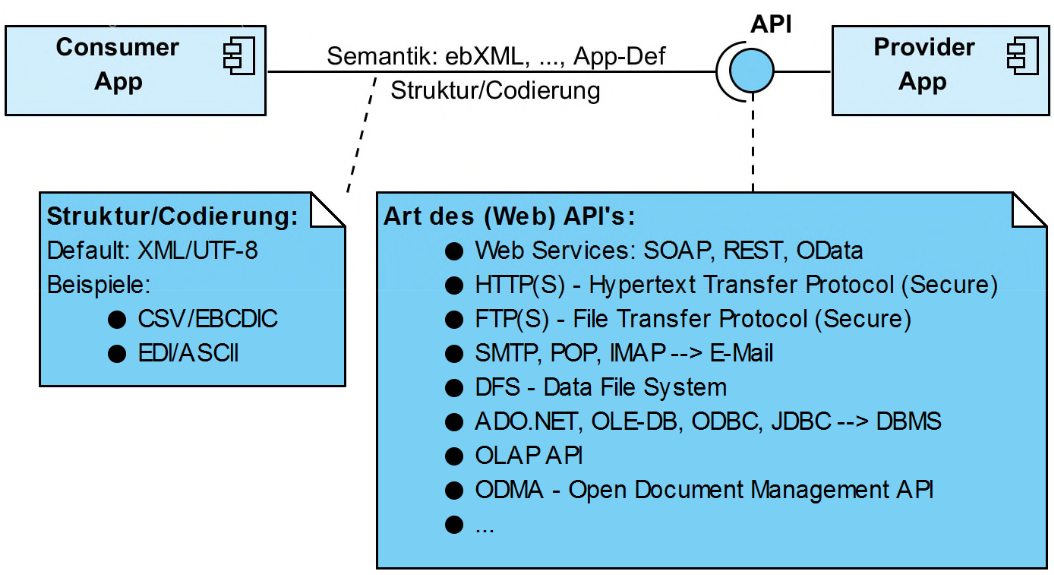
\includegraphics[width=\linewidth]{integration-draft-arch.png}

\begin{itemize}
    \item Komponente $\rightarrow$ ganze Applikation. Kann als Consumer oder Provider agieren
    \item Provider App bietet APIs an
    \item API ist mit dem höchsten Protokoll angeschrieben. Wichtigsten Varianten in der Notiz ersichtlich
    \item Consumer App hat Assoziation mit halboffenem Kreis. Beschriftung zu Semantik, Struktur und Codierung
    \item Client-App ist nur dann zu modellieren, wenn diese nicht Teil einer Gesamtapplikation ist
    \item Realtime-Verbindungen verwenden Fachapplikationen direkt
    \item EDI Integrationen sind meist via Integration Middleware zum EDI Service Provider verbunden
    \item Asynchrone Integration erfolgt über Message Broker (MOM)
\end{itemize}

\subsubsection{Referenz Integrationarchitektur}

Wichtig: eine Applikationskomponente enthält alle Schichten (d.h. Client und Server-
Komponenten)!

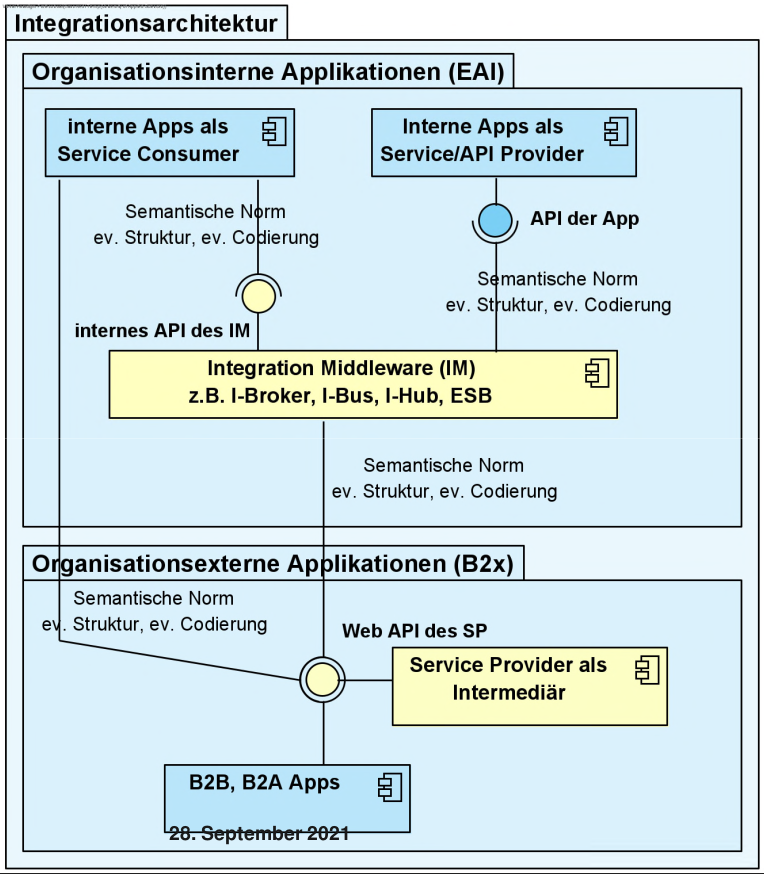
\includegraphics[width=\linewidth]{integration-reference-architecture.png} \\

\textbf{Beispiel}

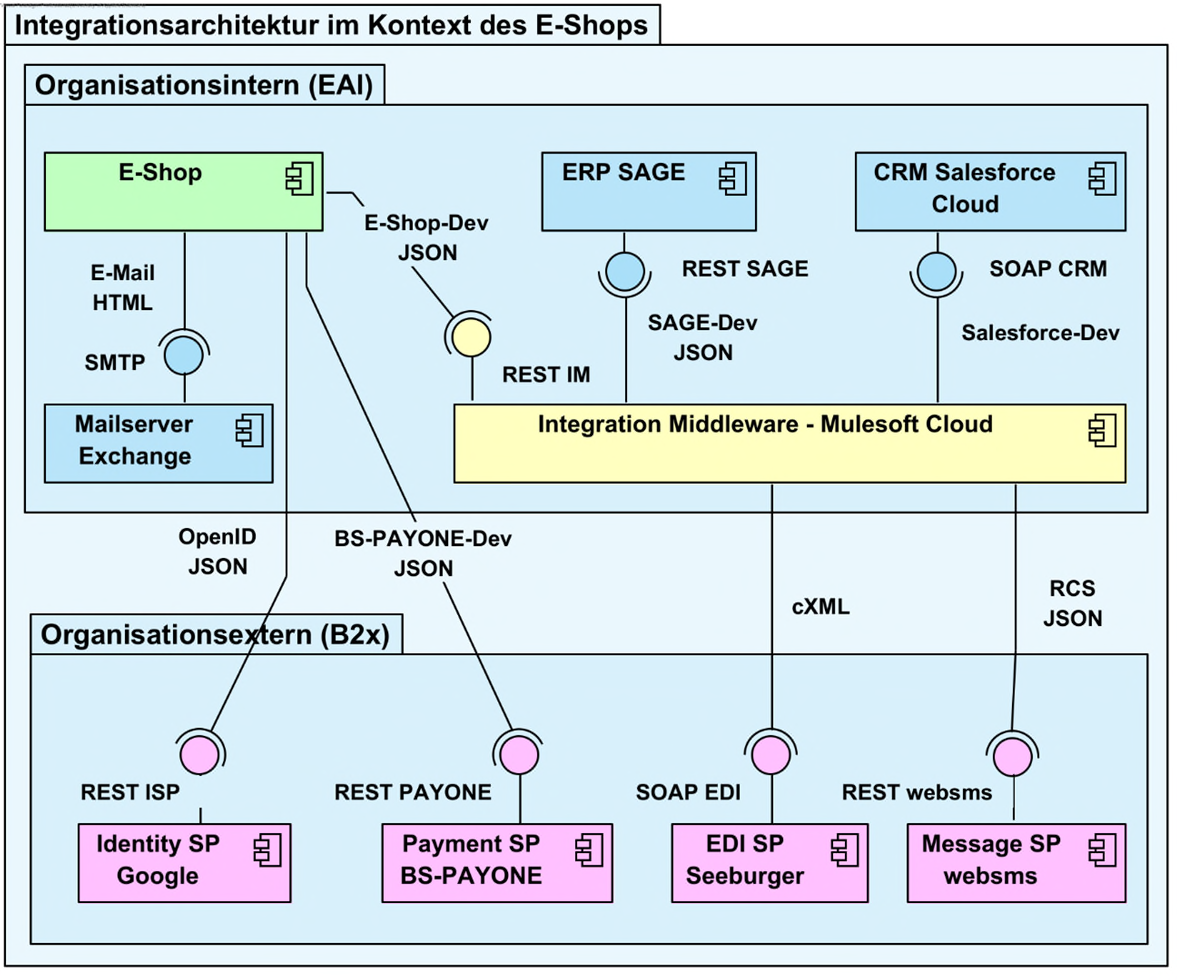
\includegraphics[width=\linewidth]{integration-example.png}

\begin{itemize}
    \item E-Shop sendet E-Mails über SMTP-Schnittstelle des Exchange-Mailservers
    \item Als alternatives Login können die Kunden Google als Identity Provider verwenden
    \item Zahlungsabwicklung läuft über BS-PAYONE
    \item Periodischer Datenaustausch mit internen Systemen, wie ERP und CRM erfolgt über eine REST-Schnittstelle
    \item cXML-Messages mit den Kunden über Integration Middleware zur SOAP-Schnittstelle des EDI Service Providers.
    \item WhatsApp und SMS gehen über Mulesoft zum Message Service Provider
\end{itemize}

